\begin{frame}
    \frametitle{Zeitstempel}
    \begin{center}
      \only<1>{
        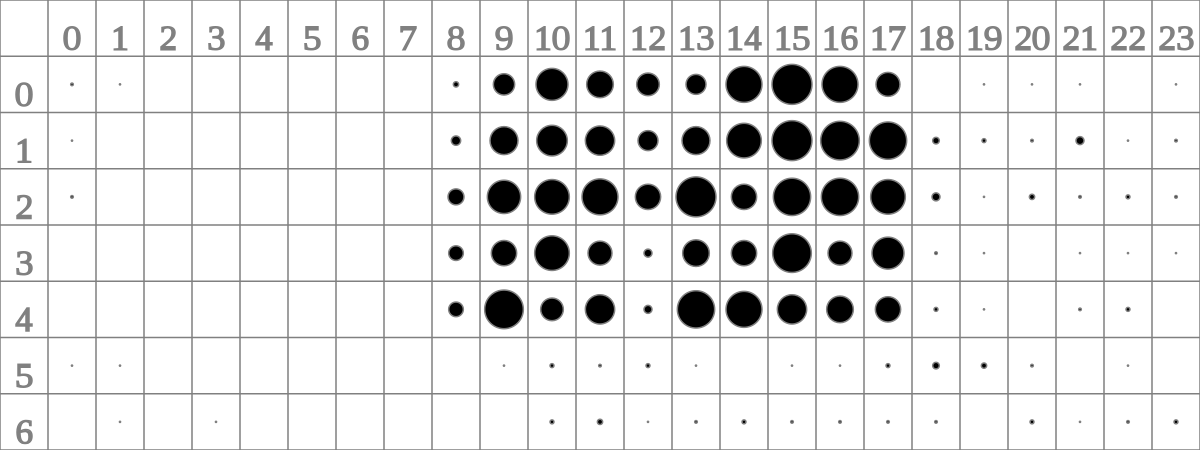
\includegraphics[width=0.9\textwidth]{img/punch_1.png}
        \\ \hfill \small Alan, Microblogging
      }

      \only<2>{
        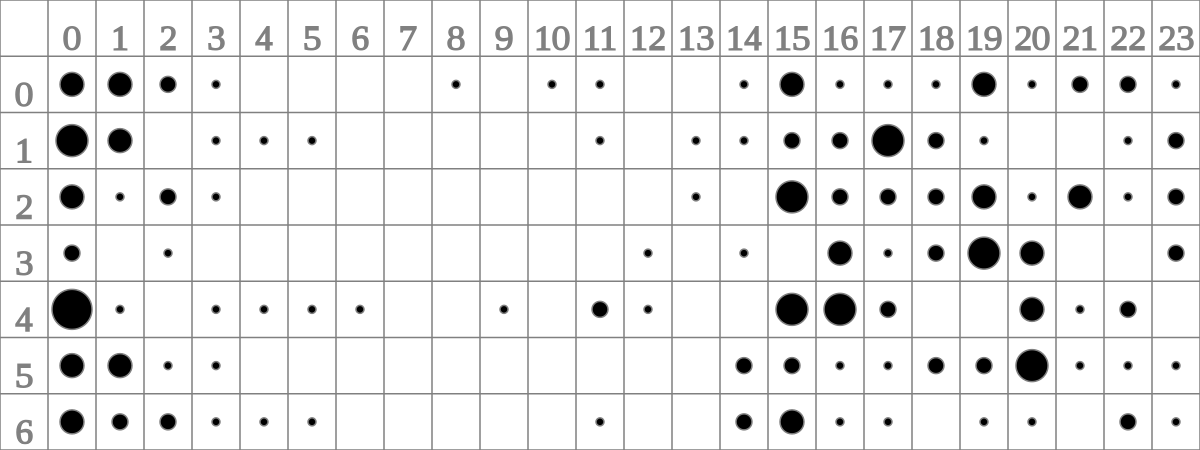
\includegraphics[width=0.9\textwidth]{img/punch_2.png}
        \\ \hfill \small Bob, Microblogging
      }

      \only<3>{
        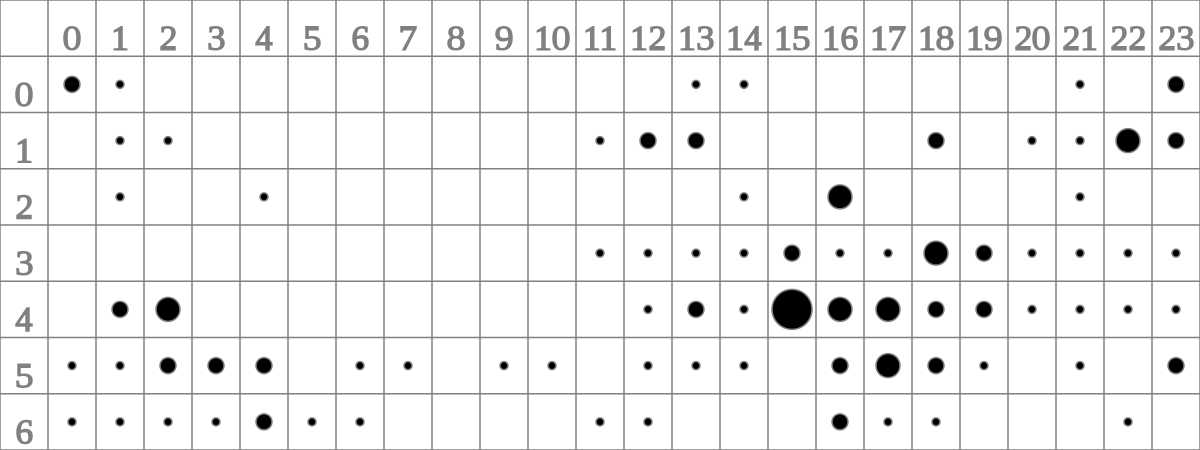
\includegraphics[width=0.9\textwidth]{img/punch_3.png}
        \\ \hfill \small Charlie, Github
      }
    \end{center}
\end{frame}

\note{Selbst anhand von Zeitmetadaten kann man eine Menge herausfinden. Hier haben wir Leute aus unserem Umfeld online ``beschattet''. Immer wenn sie bei einem sozialen Netzwerk als Online markiert waren oder aktiv etwas gepostet haben, haben wir das mitgeschnitten. Bei ``Alan'' (Name natürlich geändert) sieht man, dass er exakt während seiner Arbeitszeiten (Mo-Fr 09-17) seinen privaten Social Media Account nutzt. Bob dagegen ist eher nachtaktiv und Vormittags nicht ansprechbar. Und Charlie ist am Anfang der Woche noch halbwegs Internetabstinent, danach bricht es aber ein.}
